\documentclass[10pt]{article}
\usepackage[paperwidth=24in,paperheight=38in,margin=1.15in]{geometry}
\usepackage{graphicx}
\usepackage{booktabs}
\usepackage{amsmath}
\usepackage{array}
\usepackage{xcolor}
\usepackage{eso-pic}
\usepackage{tikz}
\usepackage{lmodern}
\pagestyle{empty}
\setlength{\parindent}{0pt}
\setlength{\parskip}{0.28cm}

\definecolor{primary}{RGB}{0,82,147}
\definecolor{secondary}{RGB}{200,16,46}
\definecolor{accent}{RGB}{0,115,120}
\definecolor{softgray}{RGB}{245,247,250}
\definecolor{linegray}{RGB}{190,198,208}

\newcolumntype{L}[1]{>{\raggedright\arraybackslash}p{#1}}
\newcommand{\HP}{\mathrm{HP}}
\newcommand{\ATK}{\mathrm{ATK}}
\newcommand{\DEF}{\mathrm{DEF}}

\AddToShipoutPictureBG*{%
  \AtPageLowerLeft{%
    
\includegraphics[width=\paperwidth,height=\paperheight]{background.pdf}%
  }%
}

\graphicspath{{../report/iclr_mota_202606/figures/}}

\newsavebox{\posterblockbox}
\long\def\posterblock#1#2#3{%
  \vspace{0.28in}
  \noindent
  \setlength{\fboxsep}{0pt}%
  \setlength{\fboxrule}{0.7pt}%
  \sbox{\posterblockbox}{%
    \begin{minipage}{\linewidth}
      \colorbox{#1}{%
        \parbox{\dimexpr\linewidth-2\fboxsep}{%
          \vspace{0.10in}
          \hspace{0.18in}{\color{white}\bfseries\Large #2}
          \vspace{0.10in}
        }%
      }%
      \vspace{0.16in}
      \hspace{0.22in}
      \begin{minipage}{\dimexpr\linewidth-0.44in}
        #3
      \end{minipage}
      \vspace{0.18in}
    \end{minipage}%
  }%
  \fcolorbox{linegray}{white}{\usebox{\posterblockbox}}%
}

\begin{document}
\fontsize{14}{17}\selectfont

\vspace*{1.35in}

\begin{center}
{\fontsize{54}{62}\selectfont\bfseries\color{primary}
Potential-Guided Planning in Magic Tower}\\[0.20in]
{\fontsize{30}{36}\selectfont\bfseries
A Deterministic Long-Horizon Resource-Allocation Benchmark}\\[0.32in]
{\fontsize{20}{25}\selectfont
Bingsong Tong (2025310812), Zhizhou Qu (2025310268), Rui Chen (2025211105)}\\[0.12in]
{\fontsize{17}{22}\selectfont Deep Reinforcement Learning Course Project 2026}
\end{center}

\vspace{0.35in}

\begin{minipage}[t]{0.485\linewidth}

\posterblock{primary}{Problem: deterministic but hard}{
Magic Tower is a fully observable single-agent RPG puzzle.  Its difficulty is
not stochasticity, but irreversible resource scheduling over HP, ATK, DEF,
keys, money, doors, items, events, and enemies.
\[
  \mathcal M =
  (\mathcal S,\mathcal A_{\mathrm{valid}}, f, r_{\mathrm{task}},
  \gamma,\rho_0,\mathcal G,\mathcal F,H).
\]
\[
  V^*(s)=
  \max_{a\in\mathcal A_{\mathrm{valid}}(s)}
  \left[r(s,a)+\gamma V^*(f(s,a))\right].
\]
\begin{itemize}
  \item Local feasibility is misleading: a legal action can destroy a future route.
  \item Combat is threshold-sensitive; one ATK/DEF point can change many future losses.
  \item Terminal reward is sparse; random exploration rarely observes success.
\end{itemize}
}

\posterblock{primary}{Environment and macro-action interface}{
\begin{center}
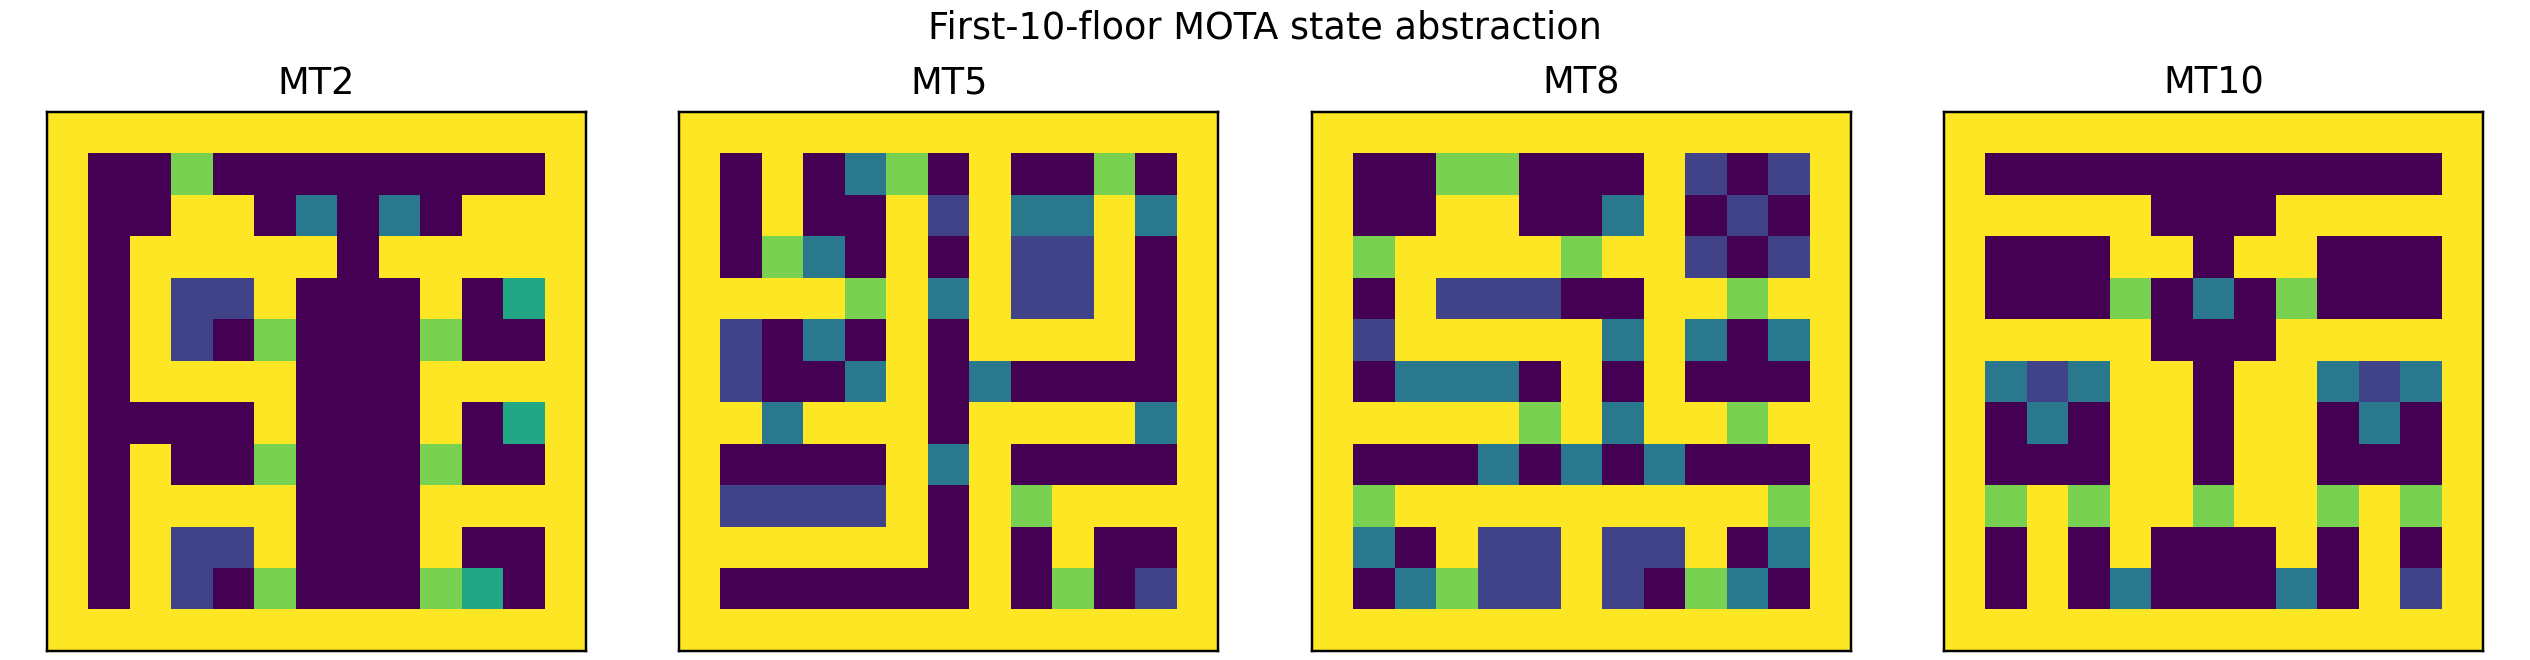
\includegraphics[width=0.92\linewidth]{mota_floor_snapshots.png}
\end{center}
We use a deterministic simulator and macro-actions over interaction nodes.
Ordinary movement is hidden inside the transition function, while
resource-changing decisions remain explicit.
\[
  \mathcal A_{\mathrm{macro}}(s)=
  \{a_i:i\in I_f, i\in R_f(s)\}
  \cup
  \{a_j:j\in \partial R_f(s), L(s,j)=1\}.
\]
Reachability is accelerated using static floor topology, interaction-node
tables, blocker bitsets, cached BFS, and lazy path reconstruction.
}

\posterblock{accent}{Potential-based reward shaping}{
Reference routes estimate a stage-conditioned potential, not a replacement for
terminal evaluation:
\[
  r_{\mathrm{search}}(s,g,a,s',g') =
  r_{\mathrm{task}}(s,a,s')
  +\lambda\bigl[\gamma\Phi_\phi(s',g')-\Phi_\phi(s,g)\bigr].
\]
\[
  \Phi_\phi(s,g)=
  \sum_k w_{g,k}c_k(s;g)+\sum_k w_k^{\mathrm{global}}c_k(s;g).
\]
Factors include hero resources, key pressure, reachable and blocked resources,
enemy damage, ATK/DEF threshold drops, stage progress, and terminal HP margin.
}

\posterblock{primary}{Three complementary approaches}{
\begin{enumerate}
  \item \textbf{Reference-route construction}: audited trajectories validate
  simulator semantics and expose feasible resource schedules.
  \item \textbf{AlphaGo Zero-style planning}: graph policy/value learning,
  single-agent PUCT-MCTS, and potential-shaped returns guide legal action search.
  \item \textbf{Multi-agent reference planner}: specialized modules score the
  same legal candidates; a beam arbiter combines stage, resource, combat, and
  terminal-objective reasoning.
\end{enumerate}
}

\end{minipage}
\hfill
\begin{minipage}[t]{0.485\linewidth}

\posterblock{primary}{Planning system}{
\begin{center}
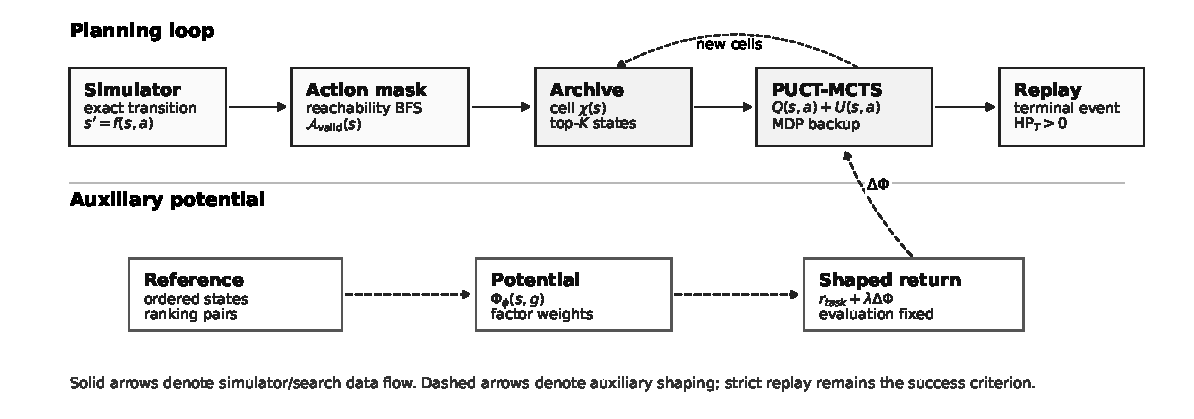
\includegraphics[width=0.96\linewidth]{system_diagram.pdf}\\[0.18in]
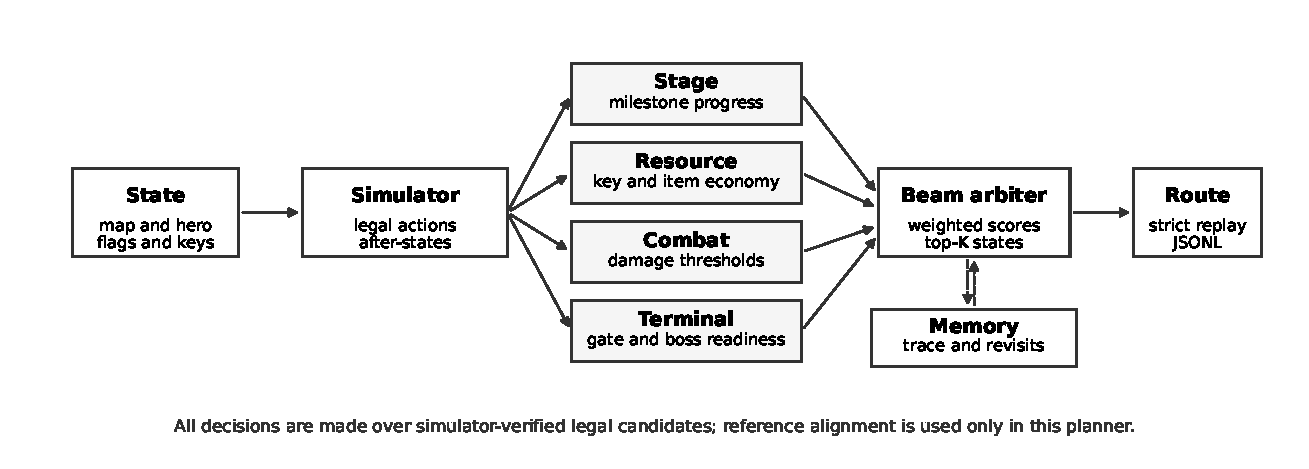
\includegraphics[width=0.96\linewidth]{agentic_architecture.pdf}
\end{center}
}

\posterblock{primary}{Policy/value model and PUCT}{
The graph policy/value model encodes interaction nodes and outputs a masked
action prior and scalar value:
\[
  f_\theta(G_s,g)=
  \left(p_\theta(\cdot\mid s,g), v_\theta(s,g)\right).
\]
PUCT selection in the single-agent setting uses
\[
  a=\arg\max_{a\in\mathcal A_{\mathrm{valid}}(s)}
  \left[
  Q(s,a)+c_{\mathrm{puct}}P(s,a)
  \frac{\sqrt{\sum_b N(s,b)}}{1+N(s,a)}
  \right].
\]
Backups accumulate deterministic task return over a max tree.
}

\posterblock{secondary}{Empirical results}{
\begin{center}
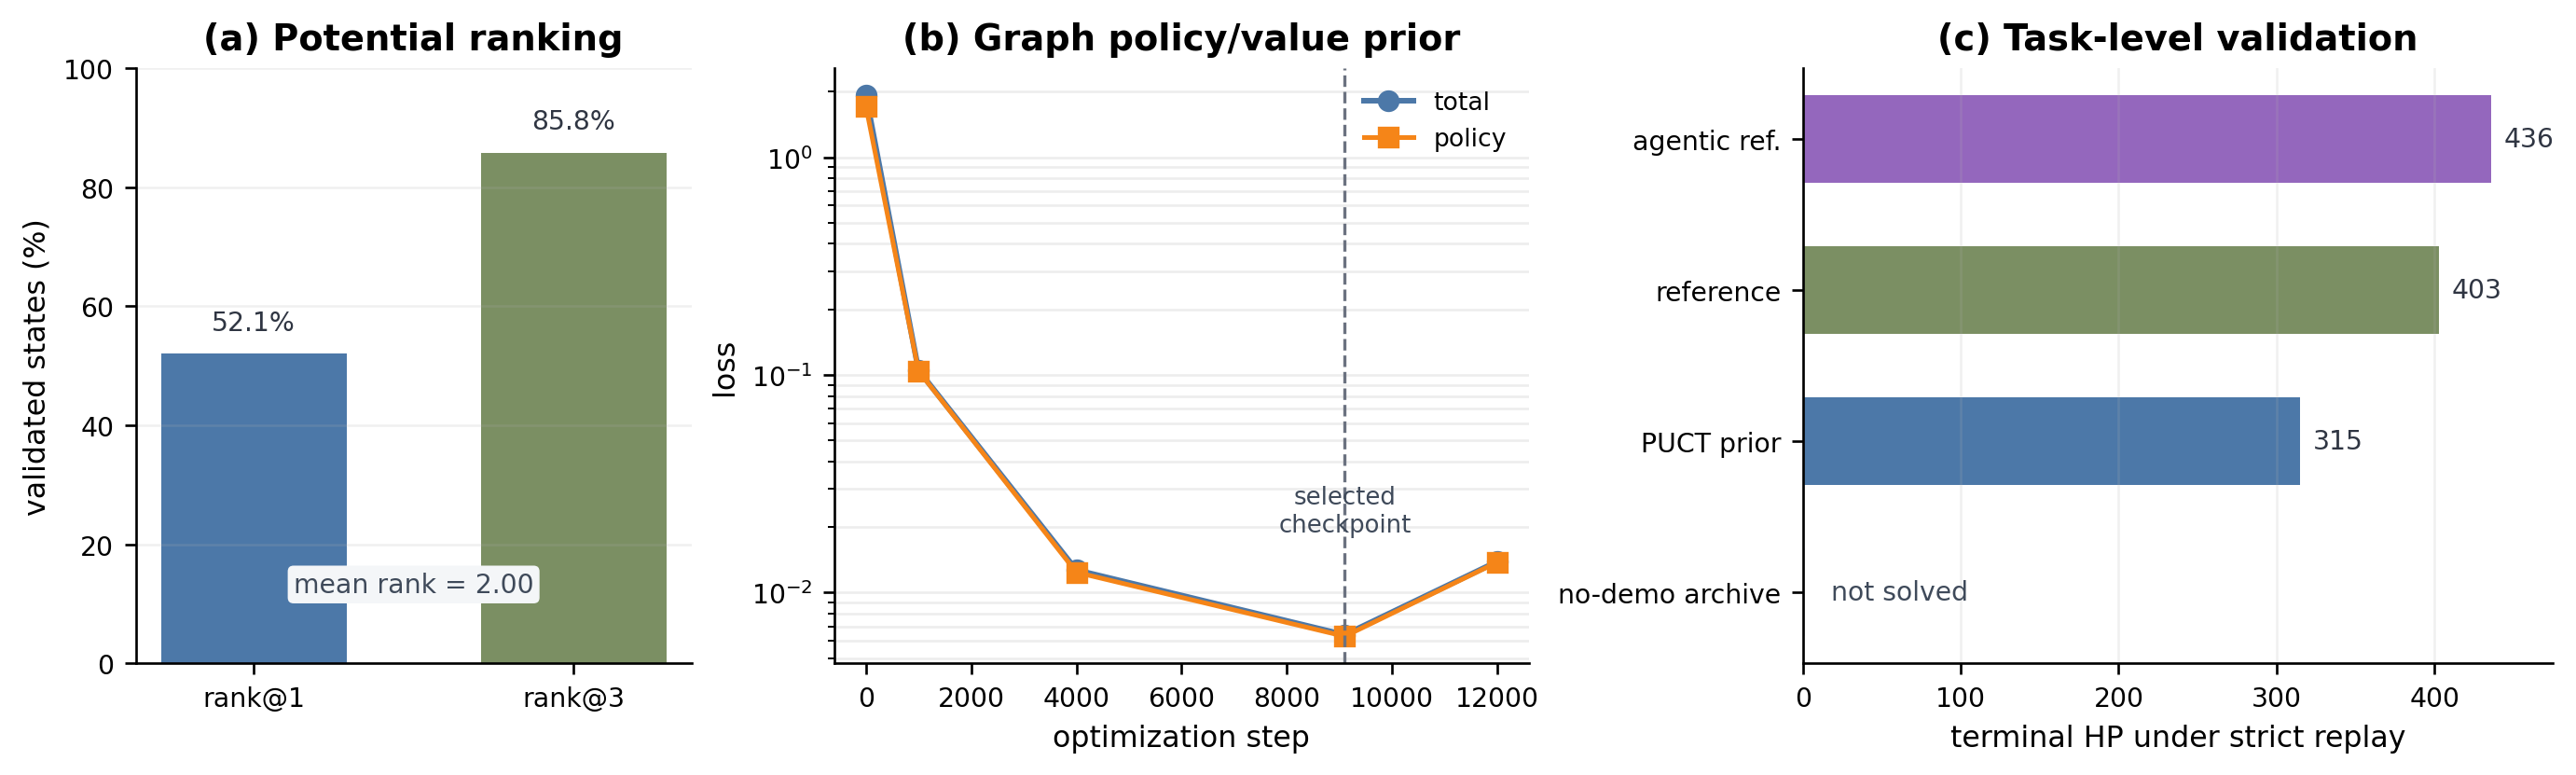
\includegraphics[width=0.96\linewidth]{experiment_summary.png}
\end{center}
\vspace{-0.12in}
\begin{center}
\begin{tabular}{L{0.34\linewidth}L{0.23\linewidth}L{0.28\linewidth}}
\toprule
Condition & Signal & Outcome\\
\midrule
Reference validation & strict replay & terminal success, \(\HP_T=403\)\\
Potential shaping & ranking & Rank@1 \(52.1\%\), Rank@3 \(85.8\%\)\\
Policy/value search & PUCT & terminal success, \(\HP_T=315\)\\
Multi-agent planner & beam search & 291 macro-actions, \(\HP_T=436\)\\
No-demonstration archive & exploration & milestones reached, terminal incomplete\\
\bottomrule
\end{tabular}
\end{center}
}

\posterblock{primary}{Route structure}{
\begin{center}
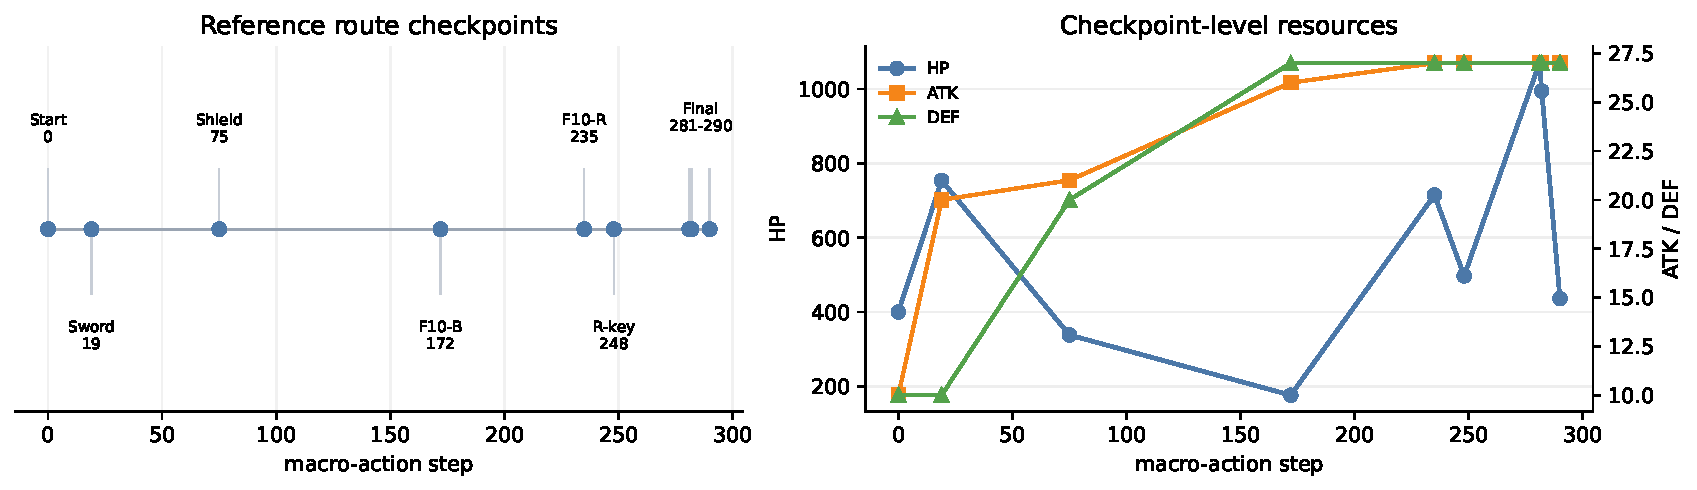
\includegraphics[width=0.96\linewidth]{agentic_route_summary.pdf}
\end{center}
The multi-agent route reaches the sword at step 19, shield at step 75,
Floor-10 resource milestones before the terminal stage, red key at step 248,
and terminal success at step 290.  It deliberately trades HP for ATK/DEF
thresholds, then rebuilds the terminal HP margin.
}

\posterblock{accent}{Benchmark outlook}{
Magic Tower can become a benchmark for long-horizon LLM and multimodal agents:
\begin{itemize}
  \item synchronized symbolic JSON, natural-language summaries, and video frames;
  \item simulator-grounded actions with strict deterministic replay;
  \item thousands of community tower instances and many walkthrough episodes;
  \item tracks for trajectory modeling, offline RL, reward learning, and
  held-out map generalization.
\end{itemize}
The multi-agent planner gives a minimal protocol for coordinated agent
reasoning over a shared candidate-action table.
}

\end{minipage}

\end{document}
